
\section{Introduction to the Architecture}

\subsection{Abstract Hardware Architecture}

For proper understanding of openETCS API and of constraints imposed on
both sides of the API, we need to define a \emph{reference abstract hardware architecture}. This hardware architecture is ``abstract''
is the sense that the actual vendor specific hardware architecture
might be totally different of the abstract architecture described in
this chapter. For example, several units might be grouped together on
the same processor.

However, the actual vendor specific architecture shall fulfill all the
requirements and constraints of this reference abstract hardware
architecture and shall not request additional constraints.

\subsection{Definition of the Reference Abstract Hardware Architecture}

\begin{figure}
  \centering
  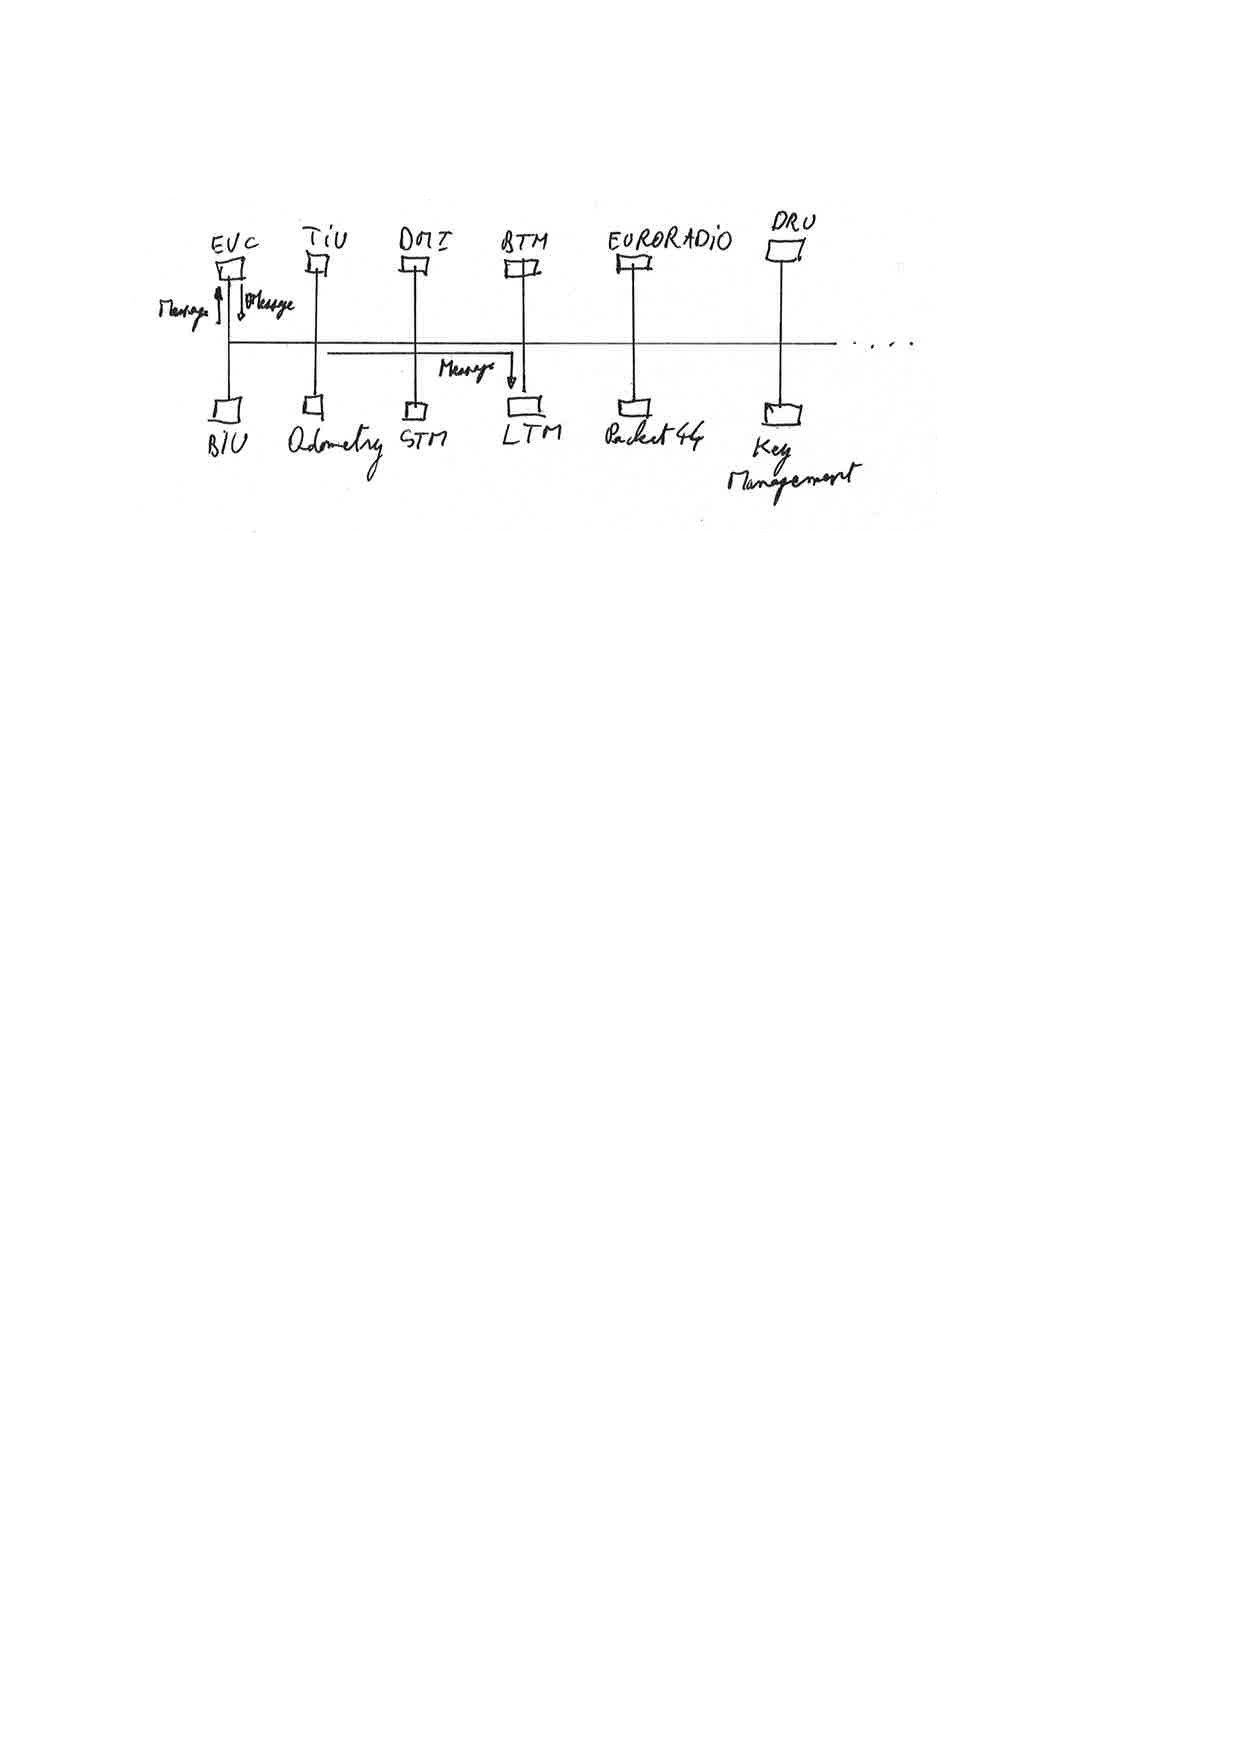
\includegraphics[width=\textwidth]{abstract-hardware-architecture.pdf}
  \caption{Reference abstract hardware architecture.}
  \label{fig:hardware-arch}
\end{figure}

The reference abstract hardware architecture is shown in Figure
\ref{fig:hardware-arch}. The reference abstract hardware architecture is made of a bus on which are connected \emph{units} defining the OBU:
\begin{itemize}
\item {EVC};
\item {TIU};
\item {ODO};
\item {DMI};
\item {STM};
\item {BTM};
\item {LTM}: Not part of this openETCS implementation;
\item EURORADIO;
\item {JRU}: Not part of this openETCS implementation;
\end{itemize}

Elements not being part of this implementation are marked. Those units shall working concurrently. They shall exchange information with other units through asynchronous message passing.

\subsection{Reference Abstract Software Architecture}
\label{software-arch}

\begin{figure}
  \centering
  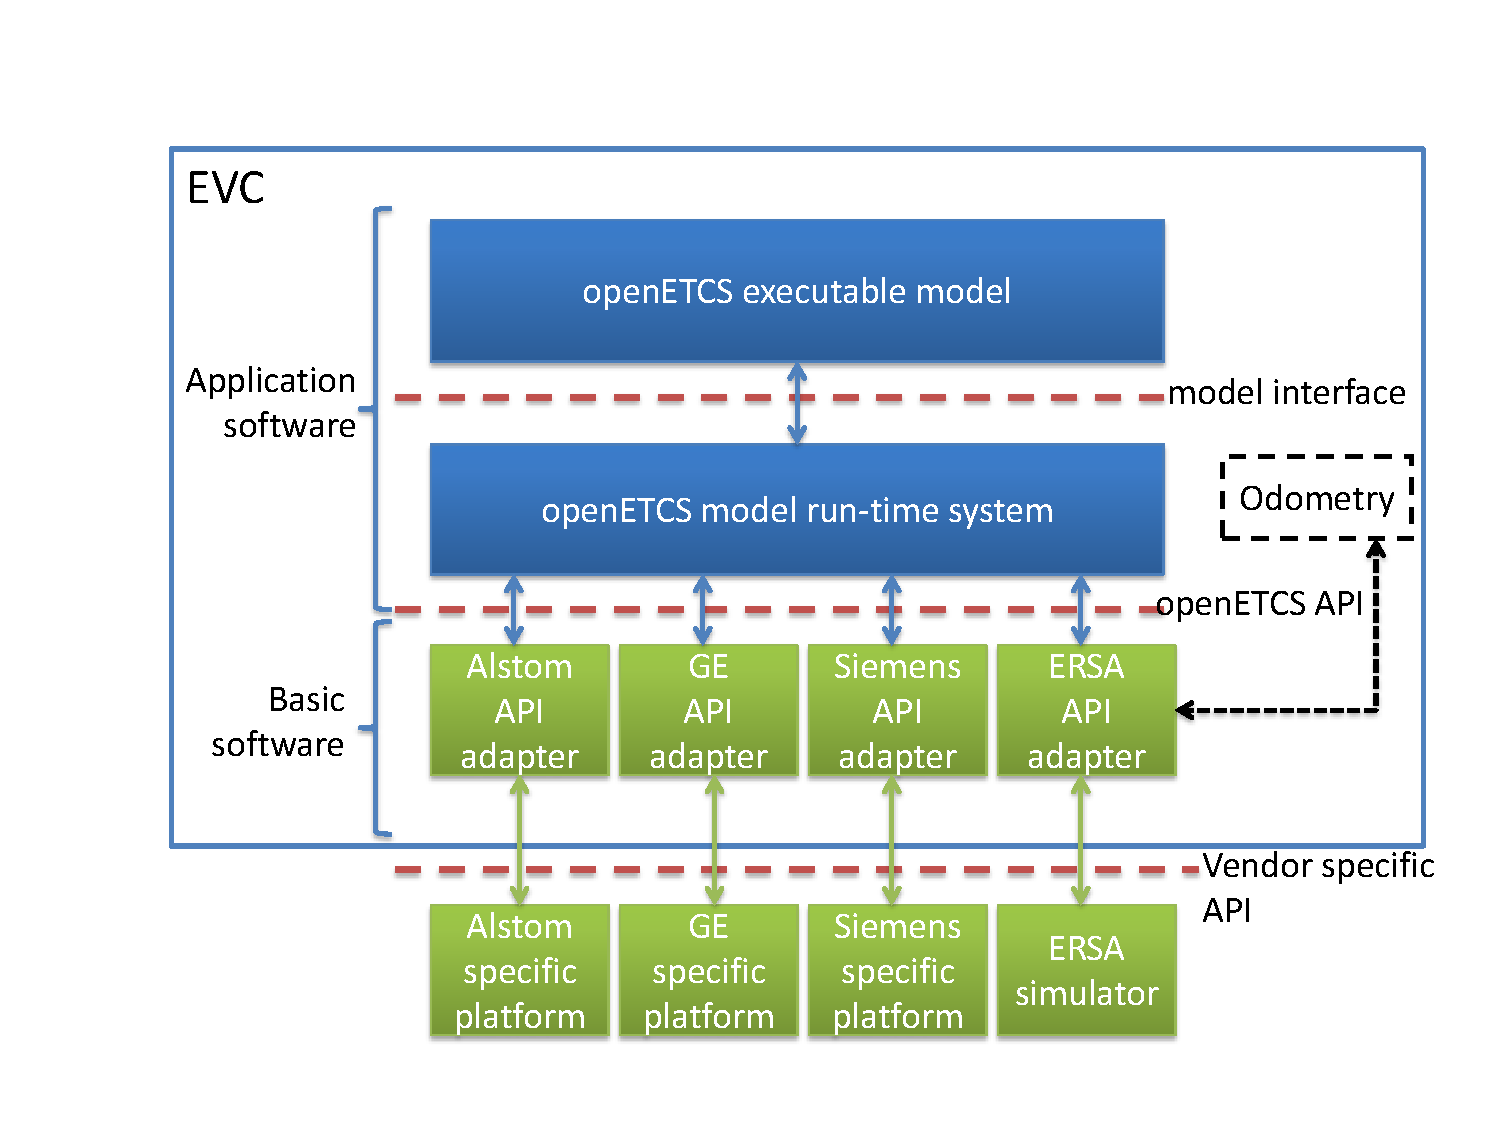
\includegraphics[width=0.9\textwidth]{software-architecture.pdf}
  \caption{Reference abstract software architecture}
  \label{fig:software-arch}
\end{figure}

The \emph{reference abstract software architecture} is shown in Figure
\ref{fig:software-arch}. This architecture consists of following
elements:
\begin{description}
\item[openETCS executable model] produced by the SCADE model \cite{scade-model}. It shall contain the program implementing core
  ETCS functions;
\item[openETCS model run-time system] shall help the execution
  of the openETCS executable model by providing additional functions
  like encode/decode messages, proper execution of the model through
  appropriate scheduling, re-order or prioritize messages, etc. 
\item[Vendor specific API adapter] shall make the link between
  the Vendor specific platform and the openETCS model run-time system.
  It can buffer message parts, encode/decode messages, route messages
  to other EVC components, etc.
\item[EVC] All above three elements shall be included in the EVC;
\item[Vendor specific platform] shall be all other elements of
  the system, bus and other units, as shown in Figure \ref{fig:hardware-arch}.
\end{description}

We have thus three interfaces:
\begin{description}
\item[Model interface]
 is the interface between openETCS executable model and openETCS model run-time system. 
\item[openETCS {API}]
 is the interface between openETCS model run-time system and Vendor specific {API} adapter.
\item[Vendor specific {API}]
 is the interface between Vendor specific {API} adapter and Vendor specific platform. This interface is not publicly described for all vendors. You can find the Alstom implementation as an example.
\end{description}

The two blocks openETCS executable model and openETCS model run-time
system are making the \emph{application software} part. This application software might be either openETCS reference software or vendor specific software.

The Vendor specific API adapter is making the \emph{Basic software} part.



